\documentclass{report}

\usepackage[headings]{fullpage}
\usepackage{scribe}

% Packages
\usepackage{amsfonts}\usepackage{amsmath}
\usepackage{amsthm}
%\usepackage[letterpaper,margin=1in]{geometry}
\usepackage{epsfig}
\usepackage{color}
\usepackage{array}
\usepackage{pstricks}
\usepackage{pst-plot}
%\usepackage{pstricks-add}
\usepackage{multirow}

\theoremstyle{plain}
\newtheorem{lemma}{Lemma}
\newtheorem{claim}[lemma]{Claim}
\newtheorem{theorem}[lemma]{Theorem}
\newtheorem{corollary}[lemma]{Corollary}
\newtheorem{prop}[lemma]{Property}
\newtheorem{fact}[lemma]{Fact}

\theoremstyle{definition}
\newtheorem{define}[lemma]{Definition}
\newtheorem{example}[lemma]{Example}

\newtheorem{problem}{Problem}

\newcommand{\E}{\mathbb{E}}
\newcommand{\R}{\mathbb{R}}
\newcommand{\bP}{\mathbb{P}}
\newcommand{\var}{\mbox{\rm var}}
\newcommand{\pr}{\mbox{\rm Pr}}

\def\X{{\cal X}}
\def\cost{{\mbox{\rm cost}}}
\def\U{{\cal U}}

\begin{document}

\course{CSE 103}
\coursetitle{Probability and statistics}
\semester{Fall 2013}
\lecturer{}
\scribe{}
\lecturenumber{6}
\lecturetopic{CDFs and sorting}

\maketitle
\section{Cumulative Distribution Functions}

Our discussion so far focused on finite event spaces or event spaces
that correspond to the integers $0,1,2,\ldots$ (so-called countable
infinite sets). How do we define distributions over the real numbers?
That is an {\em uncountably} infinite set.\footnote{A set $A$ is
  uncountable if there is no one-to-one mapping from $A$ to the
  positive integers $1,2,3,4,...$. In other words, a set is
  uncountable if you cannot create a list which includes all of the
  elements in the set.}

When defining a distribution over the real it is not enough to assign
probabilities to individual points on the real line. Consider the {\em
  uniform distribution on the line segment $[0,1]$}, by which
we mean the set $\{x | 0 \leq x \leq 1\}$. We cannot assign each
point a probability larger than zero. because that would result in
$[0,1]$ an infinite probability. What we do instead is assign
probability to the line segment $0 \leq a < b \leq 1$ the probability
$b-a$. Thus for example $P([1/4,1/3])=1/3-1/4 = 1/12$.

More generally, we can define any distribution over the real line
using the {\em Cumulative Distribution Function}:
\newcommand{\CDF}{\mbox{CDF}}
\[
\CDF(a) \doteq P(x \leq a)
\]

\begin{figure}[th]
\begin{center}
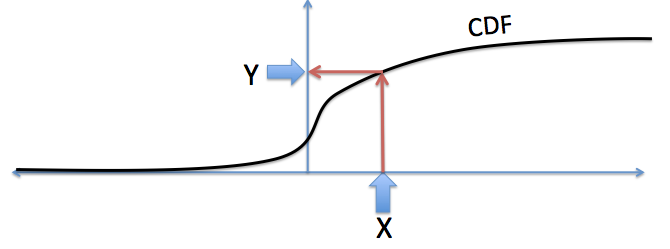
\includegraphics[width=5in]{figs/CDFmapping.png}
\end{center}
\caption{This figure depicts an example of mapping a random variable
  $X$ whose distribution is defined by a CDF (thick black curve) to
  another random variable $Y$, whose distribution is uniform in the
  interval $[0,1]$. The mapping uses the CDF as a function so that
  $Y=\CDF(X)$. \label{fig:CDFmap}}
\end{figure}

\begin{figure}[h]
\begin{center}
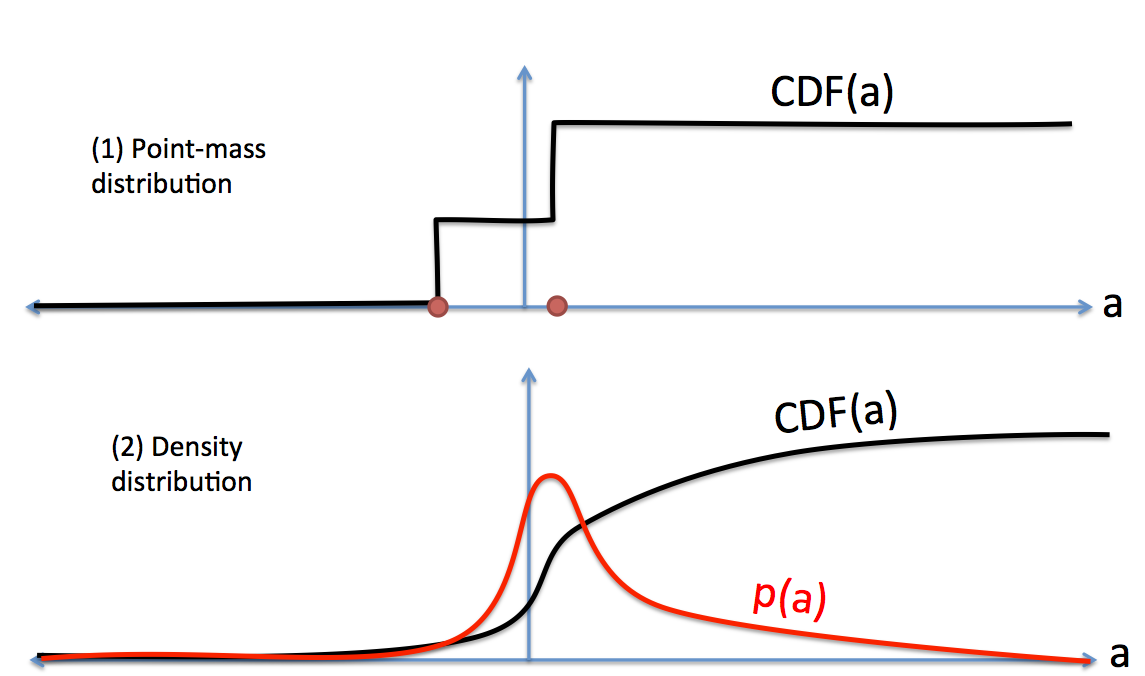
\includegraphics[width=5in]{figs/CDFs.png}
\end{center}
\caption{The CDFs for two distributions: (1) A point-mass distribution
  is a distribution that assignes non zero probabilities to two real
  values (marked by red circles) all sets that do not include at least
  one of these points have probability zero. The CDF of a point mass
  distribution is constant every where but at the point masses where
  it is discontinuous, the size of the discontinuity is the
  probability of the corresponding point. (2) A density distribution
  assigns probability zero to any single point. The CDF for such a
  distribution is a continuous increasing function that has a
  derivative. This derivative, $p(a)$ is called the {\em density function} of
  the distribution. For density distributions the CDF and the density
  function contain the same information.\label{fig:CDF}}
\end{figure}

As we see in Figure~\ref{fig:CDF} the CDF is an increasing function that
increases from zero at $-\infty$ to one at $+\infty$.

It is easy to see that $P(a<x\leq b)=\CDF(b)-\CDF(a)$.


\section{Examples of distributions on the real line}
If the distribution assigns a non-zero probability to some $x=a$ we
say that the distribution has a {\em point mass} at $a$. In that case
the $\CDF$ has a jump at $a$. We denote a point mass distribution
concentrated at the point $a$ by $PM(a)$. The distribution $PM(a)$
corresponds to a random variable such that $P(X=a)=1$.

\begin{figure}[t]
\begin{center}
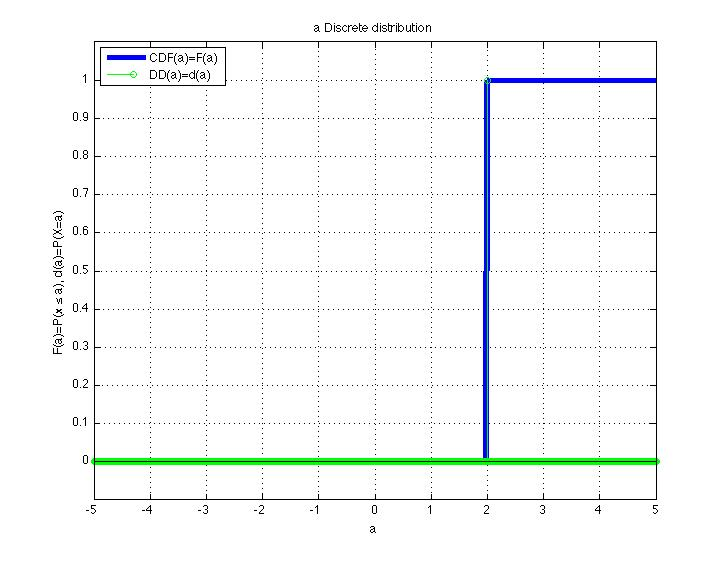
\includegraphics[width=3in]{figs/Discrete1.jpg}
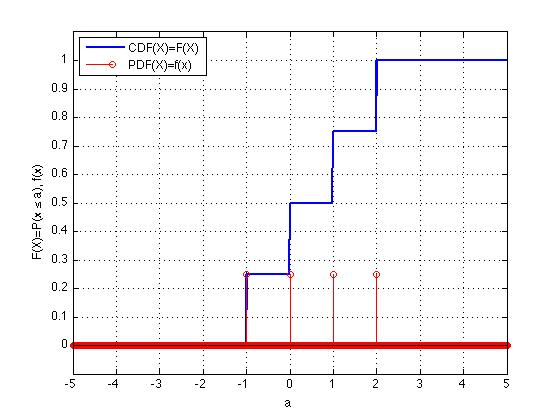
\includegraphics[width=3in]{figs/4PointMass.jpg}
\end{center}
\caption{{\bf Left:} A discrete distribution concentrated on a single
  point $P(X=2)=1$. We denote this distribution by $PM(2)$.  {\bf
    Right:} A discrete distribution distributed evenly over the four
  points $-1,0,1,2$. This distribution can be expressed as $(PM(-1)+PM(0)+PM(1)+PM(2))/4$.}
\end{figure}

\begin{figure}[b]
\begin{center}
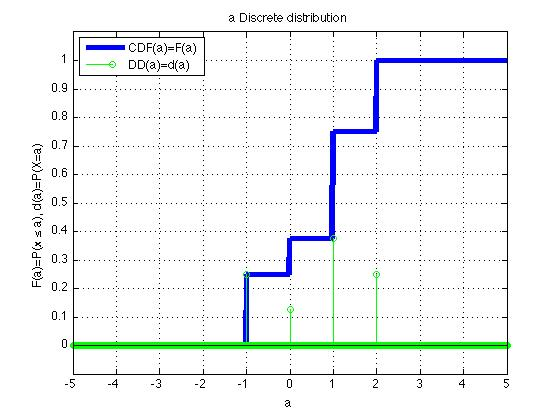
\includegraphics[width=3in]{figs/Discrete2.jpg}
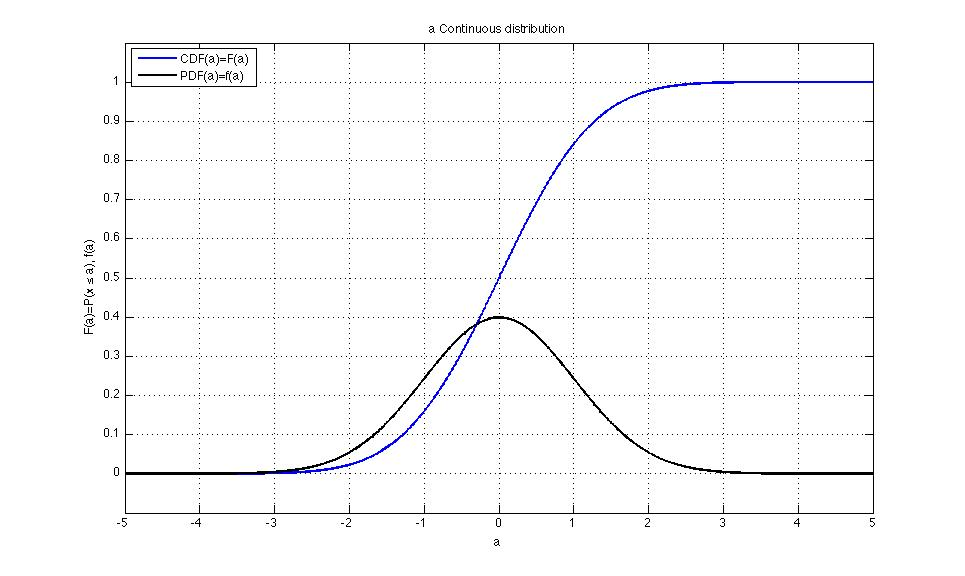
\includegraphics[width=3in]{figs/Normal.jpg}
\end{center}
\caption{{\bf Left:} A non-uniform discrete distribution. This
  distribution can be expressed as
  $(1/4)PM(-1)+(1/8)PM(0)+(5/8)PM(1)+(1/4)PM(2)$. {\bf Right:} The
  normal distribution with mean $0$ and varriance 1, denoted ${\cal
  N}(0,1)$. This is a density distribution and it's density function
is $f(x) = \frac{1}{\sqrt{2\pi}} \exp(-x^2/2)$.}
\end{figure}

\begin{figure}[t]
\begin{center}
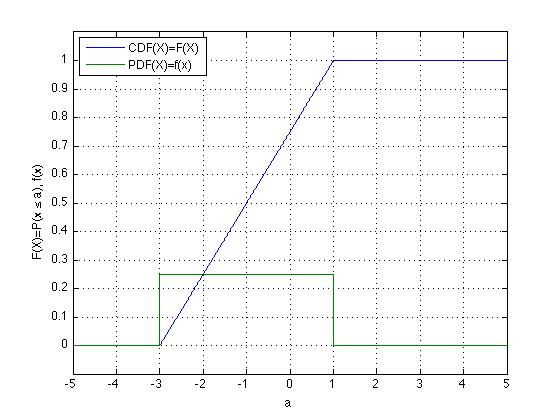
\includegraphics[width=3in]{figs/Uniform.jpg}
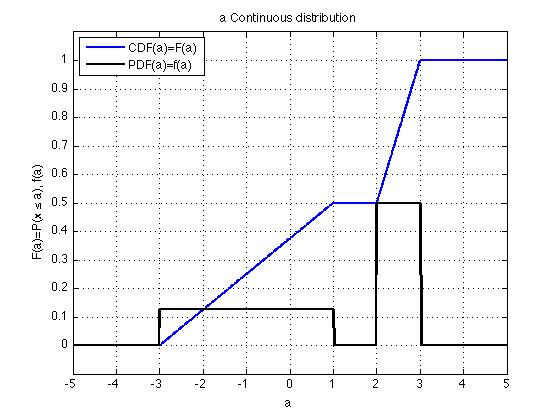
\includegraphics[width=3in]{figs/unifMixture2CDF.jpg}
\end{center}
\caption{{\bf Left:} A uniform distribution between $-3$ and $1$. We
  denote this distribution by $U(-3,1)$. {\bf Right:} A mixture of two
  uniform distributions: $(U(-3,1)+U(2,3))/2$.}
\end{figure}

\[
f(x) = \begin{cases}
0.25 & \mbox{if $ -3 \leq x \leq 1$} \\
0 & \mbox{otherwise}
\end{cases}
\]

Another important case is when the deriveative of the CDF is deifined
$p(a) = \frac{d}{dx}\left|_{x=a} \CDF(x)\right.$. The function $p(a)$
is called the {\em probability density}. Note that if $p(a)$ is
defined then, regarless of how large $p(a)$ is, $P(x=a)=0$.

When a distribution over the reals is a density distribution we can
calculate the probability of the segment $[a,b]$ using the integral:
\[
P(a < x \leq b)=\CDF(b)-\CDF(a)=\int_a^b p(x) dx
\]



\section{Sorting in expected linear time}
\label{sec:sorting}
Suppose we want to sort an array of numbers $S[1\cdots n]$ that we expect to be
distributed uniformly in some range $[\min,\max]$. Here's a {\it bucket sort} approach:
\begin{itemize}
\item Divide $[\min,\max]$ into $n$ equal-sized intervals. These are the {\it buckets} 
$B_1, B_2, \ldots, B_n$.
\item Now scan array $S$ from left to right, putting each element $S[i]$ in its
appropriate bucket.
\item Return $\mbox{sort}(B_1) \circ \mbox{sort}(B_2) \circ \cdots \circ \mbox{sort}(B_n)$,
where ``sort'' is a standard sorting algorithm (say mergesort).
\end{itemize}

Notice that there is no randomization in the algorithm. However, we can talk about
the expected running time if the elements of $S$ are generated from a uniform 
distribution over $[\min,\max]$. In that case, each element is equally likely to 
fall into any of the buckets $B_i$.

Let $N_i$ be the number of array elements that fall into $B_i$. Assuming
we use a standard sorting procedure for each bucket, we get a total running time of
$$ T = N_1 \log N_1 + N_2 \log N_2 + \cdots + N_n \log N_n \ \leq \ 
N_1^2 + N_2^2 + \cdots + N_n^2 .$$

What is $\E(N_i^2)$? The easiest way to compute this is to write $N_i$ as a sum:
$$ N_i = X_1 + X_2 + \cdots + X_n$$
where $X_j$ is 1 if the array element $S[j]$ falls into bin $i$, and 0 otherwise.
Notice that $X_j^2 = X_j$, and that $X_j$ is independent of $X_{j'}$ whenever $j \neq j'$.
Therefore,
\begin{eqnarray*}
\E(X_j)  &  = & \frac{1}{n} \\
\E(X_j^2) & = & \frac{1}{n} \\
\E(X_jX_j') & = & \E(X_j) \E(X_{j'}) \ \ = \ \ \frac{1}{n^2} \mbox{\ \ \ \ if $j \neq j'$}
\end{eqnarray*}
By linearity of expectation, we then have
\begin{eqnarray*}
\E(N_i^2) 
& = & \E \left( (X_1 + \cdots + X_n)^2 \right) \\
& = & \E \left( \sum_j X_j^2 + \sum_{j \neq j'} X_j X_{j'} \right) \\
& = & \sum_j \E(X_j^2) + \sum_{j \neq j'} \E(X_j X_{j'}) \\
& = & n \cdot \frac{1}{n} + n(n-1) \frac{1}{n^2} \ \ \leq \ \ 2.
\end{eqnarray*}

So the expected running time of the sorting algorithm, once again invoking linearity, is
$$ \E(T) 
\ \leq \ \E(N_1^2) + \E(N_2^2) + \cdots + \E(N_n^2) 
\ \leq \ 2n
.$$
It is linear!

\section{Sorting in linear time when the distribution is known}

In Section~\ref{sec:sorting} we described an algorithm that can sort
in linear time. In this section we show how to generalize this to
sorting elements drawn IID from an arbitrary density function over the reals.

Suppose we use the CDF as a transformation, in other words, map each
$X$ to $Y=\CDF(X)$. $Y$ is a new random variable, see
figure~\ref{fig:CDFmap}. What is the distribution of the random
variable $Y$? First, it is clear that $0 \leq Y \leq 1$ because that
is the range of cumulative distribution function. We need to also
assume that the CDF is a {\em reversible} function. I.e. for any real
in the range: $0<c<1$ there exists an inverse $b=\CDF^{-1}(c)$ such
that $\CDF(b)=c$. A sufficient condition for this to hold is that the
distribution over $R$ is defined by a density function.

To understand the distribution of $Y$, let us calculate the
probability that $Y$ is in some range $c<Y<d$, where $0<c<d<1$.
Using the definition of $\CDF^{-1}$ we get
\begin{equation} \label{eqn:CDF}
P(c \leq Y \leq d) = P(\CDF^{-1}(c) \leq X \leq \CDF^{-1}(d)) =
\CDF(\CDF^{-1}(d))-\CDF(\CDF^{-1}(c)) = d-c
\end{equation}
Where the first equality is justified by the definition of
$\CDF^{-1}$, the second by the formula for calculating the probability
of a segment using the CDF, and the fourth by the cancellation :
$\CDF^{-1}(\CDF(X))=X$.  We find that the distribution of $Y$ is
uniform between 0 and 1, under the condition that the CDF is invertible.

It might help to consider a particular CDF as an example. Suppose the
CDF of $X$ is $\CDF(x) = \frac{1}{1+e^{-x}}$, this function is
invertible and it's inverse is
$\CDF^{-1}(y)=\ln\left(\frac{1}{y}-1\right)$. Apply the steps of
Equation~(\ref{eqn:CDF}) to convince yourself the it works.

Recall that we have an efficient algorithm for sorting numbers that
are distributed uniformly in some segment $[\min,\max]$.
If we know the CDF of the distribution that is generating the
numbers we wish to sort, we can map these numbers to the rannge
$[0,1]$ and then use the method suggested in the first section to sort
them in $O(N)$ time.

\section{Two types of randomized algorithms}

Our algorithms for finding percentiles and for sorting are guaranteed to return 
the correct answer. But if you run them multiple times on the same input, their 
running times will fluctuate, even though the answer will be the same every time. 
Therefore we are interested in their {\it expected} running time. We call these 
{\it Las Vegas algorithms}.

Sometime we are interested in a different kind of guarantee. We have a
strict bound on the running time of the algorithm, on the other hand,
the algorithm is allowed to sometimes return an incorrect answer. This
kind of randomized algorithm is called a {\it Monte Carlo algorithm}.
A monte-carlo algorithm returns the correct answer with some
probability $p>0$.
Therefore, if you run it multiple times on an input, you'll
get many different answers, of which roughly a $p$ fraction will be
correct. In many cases, it is possible to look through these answers
and figure out which one(s) are right.

In a Monte Carlo algorithm, how much does the probability of success
increase if you run it multiple times, say $k$ times?
$$ \pr(\mbox{wrong every time}) \ = \ (1-p)^k \ \leq \ e^{-pk} .$$
To make the right hand side less than some $\delta$, we take the $\ln$ (natural log)
of both sides to get $\ln \delta > -p k$, which means it is enough
to run the algorithm $(1/p) \ln (1/\delta)$
times. For instance, to make the failure probability less than 1 in a
million, just run the algorithm $14/p$ times (a million is less than
$e^{14}$).

\end{document}
